\chapter*{Exercises C7}

\begin{enumerate}
	
	\item \begin{subequations}
		To determine MLE of $ \theta $, first find the joint PDF $ f(x_1, x_2, \dots, x_n) $ \\
			\begin{align}
				f(x_1, x_2, \dots, x_n | \theta) &= \prod_{i=1}^{n} \exp(\theta-x_i) \qquad \forall\ x_i \geq \theta \nonumber \\
				%
				&= \exp \left[ \sum\limits_{i=1}^{n} (\theta - x_i) \right] = \exp \left[n\theta - \sum x_i\right] \nonumber \\
				%
				\log (f) &= n\theta - \sum x_i		
			\end{align}
		This is maximised when $ \theta $ is maximised, but $ \theta \leq x_i\ \forall i \in \{1,\dots, n\} $.
		Thus, $ \widehat{\theta} = \min(\{x_i\}) $ \\
	\end{subequations}
	
	\item \begin{subequations}
		\begin{align}
		f(x) &= 0.5\ \exp\left(-|x- \theta|\right) \qquad \forall\ x \in \mathbb{R} \nonumber \\
		%
		f(x_1, x_2, \dots, x_n | \theta) &= \frac{1}{2^n}\ \exp\left[ \sum\limits_{i=1}^{n} -|x_i - \theta| \right] \nonumber \\
		%
		\log (f) &= -n\log (2) - \sum\limits_{i=1}^{n} |x_i - \theta| 
	\end{align}
	\end{subequations} \\
	
	
	$ \sum |x_i - \theta| $ is total absolute error. This is minimized by $ \widehat{\theta} = \mathrm{median}(x_1, \dots, x_n)$\\
	
	\item $ \mu $ is known, find MLE of $ \sigma^2 $. To find joint PDF and thus likelihood function,
	
	\begin{subequations}
	\begin{align}
		f(x_1, x_2, \dots, x_n | \sigma^2) &= \left(\frac{1}{\sqrt{2\pi\sigma^2}}\right)^n\ \exp \left[\sum\limits_{i=1}^{n}\ \frac{-(x_i - \mu)^2}{2\sigma^2}\right] \nonumber \\
		%
		\log(f) &= -(n/2)\ \log(2\pi) - n\ \log(\sigma) - \left[\sum\limits_{i=1}^{n}\ \frac{(x_i - \mu)^2}{2\sigma^2}\right] \\
		%
		\frac{\mathrm{d}}{\mathrm{d} \sigma^2}\ \log(f) &= 0 \nonumber \\
		%
		0 &= -\ddfrac{n}{2\sigma^2} + \frac{\sum (x_i - \mu)^2}{2\sigma^4} \nonumber \\
		%
		\widehat{\sigma}^2 &= \frac{\sum (x_i - \mu)^2}{n} \\
		%
		\mathbb{E}\left[\widehat{\sigma^2}\right] &= 1/n \sum \mathbb{E}[(x_i - \mu)^2] = \sigma^2
	\end{align}
	\end{subequations}
	\item Pareto density function with parameters $ (a, \lambda) $. Constraint on $ a $ is that $ a \leq \min({x_i}) $.
	Let $ y = \prod\limits_{i=1}^{n} x_i $
	
	\begin{subequations}
	\begin{align}
		f(x) &= \lambda a^\lambda x^{-(\lambda+1)} \qquad \forall\ x \geq a \nonumber \\
		%
		f(x_1, x_2, \dots, x_n | a, \lambda) &= \lambda^n\ a^{n\lambda}\ y^{-(\lambda + 1)} \\
		%
		\widehat{a} &= \min(\{x_i\}) \\
		%
		\frac{\mathrm{d}}{\mathrm{d} \lambda}\ (\log f) &= \frac{n}{\lambda} + n \log (a) - \log (y) \nonumber \\
		%
		\widehat{\lambda} &= \frac{n}{\log (y) - n \log (a)}
	\end{align}
	\end{subequations}

	\item Given the three sets of RVs, with means $ \mu_1, \mu_2, (\mu_1 + \mu_2) $, and common variance $ \sigma^2 $.
	
	\begin{subequations}
	\begin{align}
		G_i(\mu_1, \mu_2) &= (x_i - \mu_1)^2 + (y_i - \mu_2)^2 + (w_i - \mu_1 - \mu_2)^2 \nonumber \\
		%
		f(x_1, y_1,w_1, \dots, x_n, y_n, w_n | \mu_1, \mu_2) &= \left(\frac{1}{\sqrt{2\pi\sigma^2}}\right)^{3n}\ \exp \left[-\sum\limits_{i=1}^{n}\ \frac{G_i(\mu_1, \mu_2)}{2\sigma^2}\right] \nonumber \\
		%
		\log(f) &= -(3n/2)\ \log(2\pi) - 3n\ \log(\sigma) \nonumber \\
		%
		&- \left[\sum\limits_{i=1}^{n}\ \frac{G_i(\mu_1, \mu_2)}{2\sigma^2}\right] \\
		%
		\frac{\mathrm{d}}{\mathrm{d} \mu_1}\ \log(f) &= 0 \nonumber \\
		%
		0 &= \frac{1}{\sigma^2}\ \sum\limits_{i=1}^{n}\ (x_i - \mu_1) + (w_i - \mu_1 - \mu_2) \nonumber \\
		%
		\overline{X} + \overline{W} &= (2\widehat{\mu_1} + \widehat{\mu_2}) \\
		%
		\overline{Y} + \overline{W} &= (\widehat{\mu_1} + 2\widehat{\mu_2}) \nonumber \\
		%
		\widehat{\mu_1} = \frac{2\overline{X} - \overline{Y} + \overline{W}}{3} \qquad &\text{and} \qquad \widehat{\mu_2} = \frac{-\overline{X} + 2\overline{Y} + \overline{W}}{3}
	\end{align}
	\end{subequations}
	
	\item The sample mean and variance of $ Y = \log(X) $ is calculated as $ \overline{Y} = 3.7319,\ S_Y^2 = 0.0508 $.
	
	\begin{subequations}
	\begin{align}
		P \left\{ D \geq v \right\} &= 0.01 \nonumber \\
		%
		P \left\{ \frac{Y - \overline{Y}}{S_Y} \geq z_{0.01}\right\} &= 0.01 \nonumber \\
		%
		Y &\geq 9.8 \qquad \to \qquad X \geq 18041.35	
	\end{align}
	\end{subequations}

	Thus, a 100-year flood has a discharge of $ 18041 $.
	
	\item $ X $ is a log-normal RV. Let $ Y = \log X $. The moment generating function leads to mean and variance.
	\begin{subequations}
	\begin{enumerate}
		\item Using the MGF of $ Y $,
		\begin{align}
			\phi_Y(t) &= \exp \left( \mu t  + \frac{\sigma^2 t^2}{2}\right) \nonumber \\
			%
			\mathbb{E}[e^{Yt}] &= \mathbb{E}[X^t] \nonumber \\
			%
			\mathbb{E}[X] &= \exp \left(\mu + \frac{\sigma^2}{2}\right)
		\end{align}
	
		\item To find variance, set $ t = 2 $,
		\begin{align}
			\mathbb{E}[X^2] &= \exp \left(2\mu + 2\sigma^2\right) \nonumber \\
			%
			\mathrm{Var}(X) &= \exp \left(2\mu + 2\sigma^2\right) - \exp \left(2\mu + \sigma^2\right)
		\end{align}
	
		\item Calculating mean travel time using the above formulae,
		find $\mu =  \overline{Y} = 45.4 $ and $ \sigma^2 = S_Y^2 = 131.82 $.
		
		\begin{align}
			\mathbb{E}[X] &= \exp \left(\mu + 0.5\sigma^2\right) = 45.56
		\end{align}
		
	\end{enumerate}
	\end{subequations}

	\item The sample mean and variance of $ Y = X + \mathcal{N} (0, 0.1^2) $ is calculated as
	 $ \overline{Y} = 3.1502,\ S_Y = 0.0092 $.
	
	\begin{subequations}
		\begin{align}
			Y &\sim \mathcal{N}(X, 0.1^2) \nonumber \\
			%
			\text{95\% confidence interval is } X &\in \left(\overline{Y} \pm\frac{\sigma\ z_{0.025}}{\sqrt{n}}\right) \nonumber \\
			%
			&= 3.1502 \pm 0.08765 = [3.0625, 3.2378] \\
			%
			\text{99\% confidence interval is } X &\in \left(\overline{Y} \pm\frac{\sigma\ z_{0.005}}{\sqrt{n}}\right) \nonumber \\
			%
			&= 3.1502 \pm 0.11519 = [3.0350, 3.2654]
		\end{align}
	\end{subequations}
	
	\item The sample mean and variance of $ Y \sim \mathcal{N} (\mu, 0.08^2) $ is calculated as
	$ \overline{Y} = 11.48$.
	
	\begin{subequations}
		\begin{align}
			\text{95\% confidence interval is } \mu &\in \left(\overline{Y} \pm\frac{\sigma\ z_{0.025}}{\sqrt{n}}\right) \nonumber \\
			%
			&= 3.1502 \pm 0.04958 = [11.4304, 11.5296] \\
			%
			\text{95\% upper confidence interval is } X &\geq \overline{Y} - \frac{\sigma\ z_{0.05}}{\sqrt{n}} \nonumber \\
			%
			&= 3.1502 - 0.04161 = [11.4384, \infty) \nonumber \\
			%
			\text{95\% lower confidence interval is } X &\leq \overline{Y} + \frac{\sigma\ z_{0.05}}{\sqrt{n}} \nonumber \\
			%
			&= 3.1502 + 0.04161 = (-\infty, 11.5216]
		\end{align}
	\end{subequations}

	\item The sample mean and variance of $ Y \sim \mathcal{N} (\mu, 11.3^2) $ is given as
	$ \overline{Y} = 74.6, n = 81$.
	
	\begin{subequations}
		\begin{align}
			\text{95\% confidence interval is } \mu &\in \left(\overline{Y} \pm \frac{\sigma\ z_{0.025}}{\sqrt{n}}\right) \nonumber \\
			%
			&= 74.6 \pm 2.0652 = [72.5348, 76.6652] 
		\end{align}
	\end{subequations}

	\item $ \overline{X_n} $ is a the mean of the first $ n $ samples. $ \sigma^2 = 1 $ \\
	\begin{subequations}
		\begin{enumerate}
			\item Find the distribution of $ X_{n+1} - \overline{X}_n $,
			\begin{align}
				\overline{X_n} &\sim \mathcal{N}(\mu, \sigma^2/n) \nonumber \\
				%
				X_{n+1} &\sim \mathcal{N}(\mu, \sigma^2) \nonumber \\
				%
				X_{n+1} - \overline{X}_n &\sim \mathcal{N}(0,1 + 1/n)
			\end{align}
			
			\item $ \overline{X_n} = 4 $,
			\begin{align}
				\text{90\% confidence interval is } X_{n+1} &\in \left(\overline{X_n} \pm \sqrt{1 + 1/n}\ z_{0.05}\right)
			\end{align}
			
		\end{enumerate}
	\end{subequations}

	\item The sample mean $ \mu $ is unknown and variance is known to be $ \sigma^2 $. For a $ 100(1-\alpha) $ lower confidence interval \\
	
	\begin{subequations}
		\begin{align}
			\frac{\overline{X} - \mu}{\sigma / \sqrt{n}} &\sim Z \nonumber \\
			%
			P \left\{\frac{\overline{X} - \mu}{\sigma / \sqrt{n}} > z_\alpha\right\} &= 1 - \alpha\\
			%
			\mu &< \overline{X} + \frac{z_\alpha\ \sigma}{\sqrt{n}} \nonumber \\
			%
			\mu &\in \left(-\infty\ ,\ \overline{X} + \frac{z_\alpha\ \sigma}{\sqrt{n}}\right]
		\end{align}
	\end{subequations}
	
	\item The sample mean $ \mu $ is unknown and variance is known to be $ \sigma = 0.2 $. The 99\% two-sided confidence interval is
	$ \overline{Y} = 1.2, n = 20$.
	\begin{subequations}
		\begin{align}
			\mu &\in \left(\overline{Y} \pm \frac{\sigma\ z_{0.005}}{\sqrt{n}}\right) \nonumber \\
			%
			&= 1.2 \pm 0.1152 = [1.0848, 1.3152] 
		\end{align}
	\end{subequations}

	\item Using problem 13 data but with $ \sigma $ unknown and $ S^2 = 0.04 $. For a 99\% confidence interval, use $ \alpha = 0.01 $, $ \overline{Y} = 1.2, n = 20$.
	\begin{subequations}
		\begin{align}
			\mu &\in \left[ \overline{Y} - \frac{(t_{\alpha/2, n-1})\ s}{\sqrt{n}}, \ \overline{Y} + \frac{(t_{\alpha/2, n-1})\ s}{\sqrt{n}} \right] \nonumber \\
			%
			\mu &\in 1.2 \pm 0.1279 = [1.0720, 1.3279]
		\end{align}
	\end{subequations}

	\item Using problem 14 data to find one-sided 99\% confidence interval.
	\begin{subequations}
		\begin{align}
			\mu &\in \left(-\infty\ , \ \overline{Y} + \frac{(t_{\alpha, n-1})\ s}{\sqrt{n}} \right] \nonumber \\
			%
			c &= 1.2 + 0.1136 = 1.31357
		\end{align}
	\end{subequations}
	
	\item First perform a sub-sampling with $ m = 30$ and use it to find the required sample size $ n $. Normal RV with both mean and variance unknown.
	\begin{subequations}
		\begin{enumerate}
			\item Using $ m = 30 $, this subsample has variance $ S^2_m $. The interval width will then be\\
			\begin{align}
				b = 2t_{\alpha/2, m-1}\ \frac{S_m}{\sqrt{m}}
			\end{align}
			
			\item For large $ n $, this can be approximated to a standard normal RV $ Z $.
			\begin{align}
				A = 2z_{\alpha/2}\ \frac{S_m}{\sqrt{n}}
			\end{align}
	Solving for $ n $ gives the size of the full sample.
		\end{enumerate}
	\end{subequations}

	\item $ \sigma $ unknown and $ S = 6.9576 $. For a 95\% confidence interval, use $ \alpha = 0.01 $, $ \overline{Y} = 333.9958, n = 24$. Using a t-distribution with $ 23 $ DOF, which yields slightly larger intervals than a standard normal RV\\
	\begin{subequations}
		\begin{align}
			\mu &\in \left[ \overline{Y} - \frac{(t_{\alpha/2, n-1})\ s}{\sqrt{n}}, \ \overline{Y} + \frac{(t_{\alpha/2, n-1})\ s}{\sqrt{n}} \right] \nonumber \\
			%
			\mu &\in 333.9958 \pm 2.9379 = [331.0579, 336.9338] \qquad \text{95\% confidence} \nonumber \\
			%
			\mu &\in 333.9958 \pm 3.9870 = [330.0088, 337.9828] \qquad \text{99\% confidence} 
		\end{align}
	\end{subequations}

	\item $ \sigma $ unknown and $ S = 10.2127 $, $ \overline{Y} = 133.22, n = 18$. Using a t-distribution with $ 17 $ DOF, which yields slightly larger intervals than a standard normal RV\\
	\begin{subequations}
		\begin{align}
			\mu &\in \left[ \overline{Y} - \frac{(t_{\alpha/2, n-1})\ s}{\sqrt{n}}, \ \overline{Y} + \frac{(t_{\alpha/2, n-1})\ s}{\sqrt{n}} \right] \nonumber \\
			%
			\mu &\in 333.9958 \pm 4.3125 = [128.9097, 137.5347] \qquad \text{95\% confidence} \nonumber \\
			%
			\mu &\in \left(-\infty\ ,\  137.5312\right] \qquad \text{lower 95\% confidence} \nonumber \\
			%
			\mu &\in \left[128.9133\ ,\ \infty\right) \qquad \text{upper 95\% confidence}
		\end{align}
	\end{subequations}

	\item $ \sigma $ unknown and $ S = 22 $, $ \overline{Y} = 222, n = 9$. Using a t-distribution with $ 8 $ DOF, which yields slightly larger intervals than a standard normal RV\\
	\begin{subequations}
		\begin{align}
			\mu &\in \left[ \overline{Y} - \frac{(t_{\alpha, n-1})\ s}{\sqrt{n}}, \infty \right) \nonumber \\
			%
			\mu &\in \left[208.363\ ,\ \infty\right) \qquad \text{upper 95\% confidence}
		\end{align}
	\end{subequations}

	\item $ \sigma $ unknown and $ S = 800 $, $ \overline{Y} = 2200, n = 18$. Using a t-distribution with $ 15 $ DOF, which yields slightly larger intervals than a standard normal RV\\
	\begin{subequations}
		\begin{align}
			\mu &\in \left[ \overline{Y} - \frac{(t_{\alpha/2, n-1})\ s}{\sqrt{n}}, \ \overline{Y} + \frac{(t_{\alpha/2, n-1})\ s}{\sqrt{n}} \right] \nonumber \\
			%
			\mu &\in 333.9958 \pm 350.61 = [1849.3899, 2550.6101] \qquad \text{90\% confidence}
		\end{align}
	\end{subequations}

	\item $ \sigma $ unknown and $ S = 16 $, $ \overline{Y} = 320, n = 100$. Using a t-distribution with $ 99 $ DOF, which yields slightly larger intervals than a standard normal RV\\
	\begin{subequations}
		\begin{align}
			\mu &\in \left[ \overline{Y} - \frac{(t_{\alpha/2, n-1})\ s}{\sqrt{n}}, \ \overline{Y} + \frac{(t_{\alpha/2, n-1})\ s}{\sqrt{n}} \right] \nonumber \\
			%
			\mu &\in 320 \pm 3.1747 = [316.8252, 323.1747] \qquad \text{95\% confidence}
		\end{align}
	\end{subequations}
	
	\item $ \sigma $ unknown and $ S = 15.4 $, $ \overline{Y} = 330.2, n = 20$. Using a t-distribution with $ 19 $ DOF, which yields slightly larger intervals than a standard normal RV\\
	\begin{subequations}
		\begin{align}
			\mu &\in \left[ \overline{Y} - \frac{(t_{\alpha/2, n-1})\ s}{\sqrt{n}}, \ \overline{Y} + \frac{(t_{\alpha/2, n-1})\ s}{\sqrt{n}} \right] \nonumber \\
			%
			\mu &\in 330.2 \pm 7.2074 = [322.9926, 337.4074] \qquad \text{95\% confidence} \nonumber \\
			%
			\mu &\in 330.2 \pm 9.8517 = [320.3482, 340.0517] \qquad \text{99\% confidence}
		\end{align}
	\end{subequations}

	\item $ \sigma $ unknown and $ S = 840 $, $ \overline{Y} = 1220, n = 300$. Using a t-distribution with $ 299 $ DOF, which yields slightly larger intervals than a standard normal RV\\
	\begin{subequations}
		\begin{align}
			\mu &\in \left[ \overline{Y} - \frac{(t_{\alpha/2, n-1})\ s}{\sqrt{n}}, \ \overline{Y} + \frac{(t_{\alpha/2, n-1})\ s}{\sqrt{n}} \right] \nonumber \\
			%
			\mu &\in 1220 \pm 95.4395 = [1124.5605, 1315.4395] \qquad \text{95\% confidence} 
		\end{align}
	\end{subequations}

	\item from Problem 23,
	\begin{subequations}
		\begin{align}
			\mu &\in \left(-\infty\ ,\  \overline{Y} - \frac{(t_{\alpha, n-1})\ s}{\sqrt{n}} \right] \nonumber \\
			%
			\mu &\in \left(-\infty\ ,\ 1282.2896  \right] \qquad \text{upper 90\% confidence} \nonumber \\
			%
			v &= 1282.2896
		\end{align}
	\end{subequations}
	
	\item confidence interval for $ \mu $ when $ \sigma^2 $ is unknown. Using the sample mean and sample variance $ \overline{X}, S^2 $, and the observations for these statistics $ \overline{x}, s^2 $\\
	\begin{subequations}
		\begin{align}
			\frac{\overline{X} - \mu}{S/\sqrt{n}} &\sim t_{n-1} \nonumber \\
			%
			P \left\{ \frac{\overline{X} - \mu}{S/\sqrt{n}} > -t_{\alpha, n-1}\right\} &= 1 - \alpha \nonumber \\
			%
			\mu \in \left( -\infty\ ,\ \overline{x} + \frac{t_{\alpha, n-1}\ s}{\sqrt{n}} \right]
		\end{align}
	\end{subequations}
	
	\item $ \sigma $ unknown and $ S = 104.3435 $, $ \overline{Y} = 2062.75, n = 20$. Using a t-distribution with $ 19 $ DOF, which yields slightly larger intervals than a standard normal RV\\
	\begin{subequations}
		\begin{align}
			\mu &\in \left[ \overline{Y} - \frac{(t_{\alpha/2, n-1})\ s}{\sqrt{n}}, \ \overline{Y} + \frac{(t_{\alpha/2, n-1})\ s}{\sqrt{n}} \right] \nonumber \\
			%
			\mu &\in 2062.75 \pm 48.8343 = [2013.9157, 2111.5843] \qquad \text{95\% confidence} \nonumber \\
			%
			\mu &\in 2062.75 \pm 66.7511 = [1995.9989, 2129.5011] \qquad \text{99\% confidence} \nonumber \\
			%
			v &= 2022.41
		\end{align}
	\end{subequations}

	\item $ \sigma $ unknown and $ S = 8.6879 $, $ \overline{Y} = 98.67, n = 20$. Using a t-distribution with $ 19 $ DOF, which yields slightly larger intervals than a standard normal RV\\
	\begin{subequations}
		\begin{align}
			\mu &\in \left[ \overline{Y} - \frac{(t_{\alpha/2, n-1})\ s}{\sqrt{n}}, \ \overline{Y} + \frac{(t_{\alpha/2, n-1})\ s}{\sqrt{n}} \right] \nonumber \\
			%
			\mu &\in 98.67 \pm 4.0660 = [94.6039, 102.7360] \qquad \text{95\% confidence} 
		\end{align}
	\end{subequations}

	\item $ \sigma $ unknown and $ S = 0.02944 $, $ \overline{Y} = 0.55, n = 10$. Using a t-distribution with $ 9 $ DOF, which yields slightly larger intervals than a standard normal RV\\
	\begin{subequations}
		\begin{align}
			\mu &\in \left[ \overline{Y} - \frac{(t_{\alpha/2, n-1})\ s}{\sqrt{n}}, \ \overline{Y} + \frac{(t_{\alpha/2, n-1})\ s}{\sqrt{n}} \right] \nonumber \\
			%
			\mu &\in 0.55 \pm 0.02106 = [0.52894, 0.57106] \qquad \text{95\% confidence} 
		\end{align}
	\end{subequations}

	\item \begin{subequations}
		To find the PMF of $ N $, look at the CDF of $ N $ first. $ \mathbb{E}[U_i] = 1/2, \mathrm{Var}(U_i) = 1/12 $\\
	Consider $ S_n = U_1 + \dots + U_n $ and some. This is the $ n $ dimensional simplex problem.
	
	When finding the area of the $ n $-simplex, 
	
	Begin by proving the recursion formula for the volume of an $ n $ dimensional simplex. Let $ {X_i} $ be such that uniform RV $ X_i \in [0, 1] $ and the constraint $ \sum x_i  \leq 1$.
	
			Using analytical methods to find the exact asymptotic value of $ \mathbb{E}[X] $
			\begin{align}
				P\{S_1 \leq 1\} = A_1 &= P\{X_1 \leq 1\} = 1 \nonumber \\
				%
				P\{S_2 \leq 1\} = A_2 &= \int\limits_{0}^{1} \int\limits_{0}^{1-y} \mathrm{d}x\ \mathrm{d}y = \frac{1}{2}\\
				%
				P\{S_3 \leq 1\} = A_3 &= \int\limits_{0}^{1} (1-z)^2\ A_2\ \mathrm{d}z = \frac{A_2}{3} = \frac{1}{6}\\
				%
				P\{S_n \leq 1\} = A_n &= \int_{0}^{1} (1-x_n)^{n-1}\ A_{n-1}\ \mathrm{d}x_n = \frac{A_{n-1}}{n}		
			\end{align}
		
			The above factor of $ (1-x_n)^{n-1} $ arises as a result of all of the other $ n-1 $ dimensions being scaled down by a factor of $ 1-x_n $ when $ x_n > 0 $. From recursion, $ A_n = 1/n!$\\
			
			Now, using the above as a CDF of $ N $, then its PDF and expected value\\
			\begin{align}
				P\{N \leq n\} &= 1 - P\{N > n\} = A_n = 1 - \frac{1}{n!} \nonumber \\
				%
				P\{N = n\} &= P\{N \leq n\} - P\{N \leq n-1\} = \frac{n-1}{n!} \\
				%
				\mathbb{E}[X] &= \sum\limits_{i=1}^{\infty} i\ P\{N = i\} = \sum\limits_{i=0}^{\infty} \frac{1}{i!} = e 
			\end{align}
			
		
			Thus, the expected value of $ X $ converges to the natural logarithm $ e $.
		
			Using a Monte-Carlo simulation with $ n = k^2 \ \forall\ k \in [4, 99]$ \\
			
		\begin{figure}[H]
			\centering
			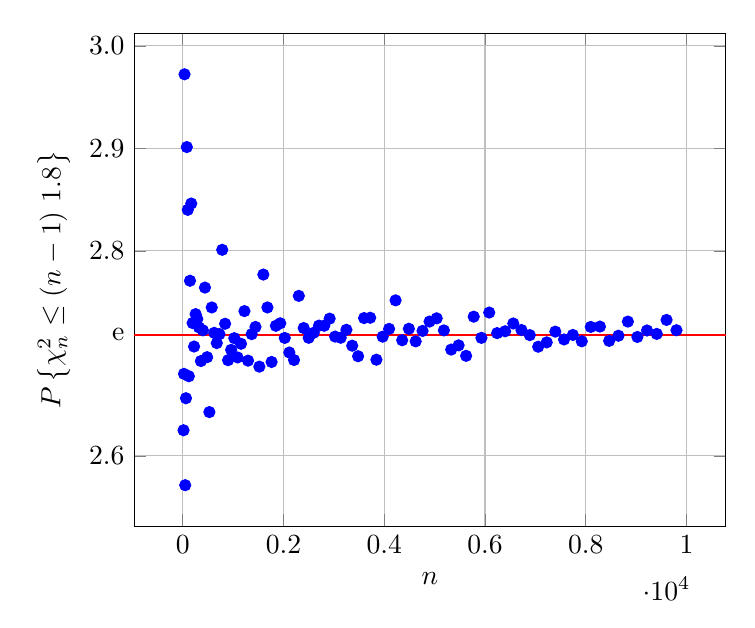
\begin{tikzpicture}
				\begin{axis}[width = 0.75\textwidth,xlabel=$n$, ylabel=$ P \left\{\chi_n^2 \leq (n-1)\ 1.8 \right\}  $, grid = both, ytick = {2.4, 2.6, e, 2.8, 2.9, 3.0}, yticklabels = {2.4, 2.6, e, 2.8, 2.9, 3.0}]
					
					\addplot[only marks, color = blue] plot coordinates{(16, 2.625) (25, 2.68) (36, 2.9722222222222223) (49, 2.5714285714285716) (64, 2.65625) (81, 2.9012345679012346) (100, 2.84) (121, 2.677685950413223) (144, 2.7708333333333335) (169, 2.8461538461538463) (196, 2.729591836734694) (225, 2.7066666666666666) (256, 2.73828125) (289, 2.7335640138408306) (324, 2.7253086419753085) (361, 2.6925207756232687) (400, 2.7225) (441, 2.764172335600907) (484, 2.696280991735537) (529, 2.6427221172022684) (576, 2.7447916666666665) (625, 2.72) (676, 2.710059171597633) (729, 2.718792866941015) (784, 2.8010204081632653) (841, 2.728894173602854) (900, 2.6933333333333334) (961, 2.7034339229968785) (1024, 2.71484375) (1089, 2.6960514233241506) (1156, 2.709342560553633) (1225, 2.7412244897959184) (1296, 2.692901234567901) (1369, 2.718772826880935) (1444, 2.7257617728531858) (1521, 2.6870479947403023) (1600, 2.776875) (1681, 2.744794765020821) (1764, 2.691609977324263) (1849, 2.7268793942671716) (1936, 2.729338842975207) (2025, 2.7150617283950615) (2116, 2.700850661625709) (2209, 2.6935264825712992) (2304, 2.756076388888889) (2401, 2.724698042482299) (2500, 2.7152) (2601, 2.7201076509034987) (2704, 2.7270710059171597) (2809, 2.7269490922036312) (2916, 2.7338820301783264) (3025, 2.7163636363636363) (3136, 2.7152423469387754) (3249, 2.7229916897506925) (3364, 2.7074910820451845) (3481, 2.697213444412525) (3600, 2.7344444444444442) (3721, 2.734748723461435) (3844, 2.693808532778356) (3969, 2.7163013353489545) (4096, 2.723876953125) (4225, 2.751715976331361) (4356, 2.7128099173553717) (4489, 2.7239919803965247) (4624, 2.7117214532871974) (4761, 2.7219071623608486) (4900, 2.7310204081632654) (5041, 2.734179726244793) (5184, 2.72241512345679) (5329, 2.70369675361231) (5476, 2.70781592403214) (5625, 2.6976) (5776, 2.735803324099723) (5929, 2.7151290268173387) (6084, 2.7398093359631823) (6241, 2.7197564492869732) (6400, 2.7215625) (6561, 2.7291571406797743) (6724, 2.7227840571088637) (6889, 2.717811003048338) (7056, 2.7064909297052155) (7225, 2.710726643598616) (7396, 2.721200648999459) (7569, 2.7135685031047694) (7744, 2.71797520661157) (7921, 2.711778815806085) (8100, 2.7258024691358025) (8281, 2.7261200338123417) (8464, 2.7121928166351608) (8649, 2.717192739044976) (8836, 2.730986871887732) (9025, 2.71601108033241) (9216, 2.7223307291666665) (9409, 2.7189924540333723) (9604, 2.7326114119117033) (9801, 2.722579328639935)};
					
					\draw [thick, draw=red,] (axis cs: -1000, e ) -- (axis cs: 11000,  e );
				\end{axis}
			\end{tikzpicture}
		\end{figure}
	\end{subequations}

	\item $ \sigma $ unknown and $ S = 3.9799 $, $ \overline{Y} = 11.5666, n = 30$. Using a t-distribution with $ 29 $ DOF, which yields slightly larger intervals than a standard normal RV\\
	\begin{subequations}
		\begin{align}
			\mu &\in \left[ \overline{Y} - \frac{(t_{\alpha/2, n-1})\ s}{\sqrt{n}}, \ \overline{Y} + \frac{(t_{\alpha/2, n-1})\ s}{\sqrt{n}} \right] \nonumber \\
			%
			\mu &\in 11.5666 \pm 1.4861 = [10.0805, 13.0528] \qquad \text{95\% confidence} 
		\end{align}
	\end{subequations}
	
	\item $ \sigma $ unknown and $ S = 9400 $, $ \overline{Y} = 90450, n = 16$. Using a t-distribution with $ 15 $ DOF, which yields slightly larger intervals than a standard normal RV\\
	\begin{subequations}
		\begin{align}
			\mu &\in \left[ \overline{Y} - \frac{(t_{\alpha/2, n-1})\ s}{\sqrt{n}}, \ \overline{Y} + \frac{(t_{\alpha/2, n-1})\ s}{\sqrt{n}} \right] \nonumber \\
			%
			\mu &\in 90450 \pm 5008.9064 = [85441.0936, 95458.9064] \qquad \text{95\% confidence} 
		\end{align}
	\end{subequations}

	\item Find the mean squared error of the predictor $ \overline{X} $,
	\begin{subequations}
		\begin{align}
			\overline{X_n} &\sim \mathcal{N}(\mu, \sigma^2/n) \nonumber \\
			%
			X_{n+1} &\sim \mathcal{N}(\mu, \sigma^2) \nonumber \\
			%
			Y = X_{n+1} - \overline{X_n} &\sim \mathcal{N}(0, \sigma^2\ (1+1/n))\nonumber \\
			%
			\mathbb{E}[Y^2] &= \mathrm{Var}(Y) + \left(\mathbb{E}[Y]\right)^2 = \sigma^2\ \left(1+\frac{1}{n}\right)
		\end{align}
	\end{subequations}

	\item $ \sigma $ unknown and $ S = 0.3775 $, $ \overline{Y} = 4.725, n = 4$. Using a t-distribution with $ 3 $ DOF, which yields slightly larger intervals than a standard normal RV\\
	\begin{subequations}
		\begin{align}
			\frac{X_{n+1} - \overline{X}_n}{S_n \sqrt{1 + 1/n}} &\sim t_{n-1} \nonumber \\
			%
			\mu &\in \left[ \overline{Y} - (t_{\alpha/2, n-1})\ s \sqrt{1 + 1/n}, \ \overline{Y} + (t_{\alpha/2, n-1})\ s \sqrt{1 + 1/n} \right] \nonumber \\
			%
			\mu &\in 4.725 \pm 1.3431 = [3.3818, 6.0681] \qquad \text{95\% confidence} 
		\end{align}
	\end{subequations}
	
	\item  $ \sigma $ unknown and $ S = 2.12 $, $ \overline{Y} = 2.5, n = 30$. Using a t-distribution with $ 29 $ DOF, which yields slightly larger intervals than a standard normal RV,
	\begin{subequations}
		\begin{align}
			\mu &\in \left(-\infty\ ,\  \overline{Y} - \frac{(t_{\alpha, n-1})\ s}{\sqrt{n}} \right] \nonumber \\
			%
			\mu &\in \left(-\infty\ ,\ 3.0076  \right] \qquad \text{upper 90\% confidence} \nonumber \\
			%
			v &= 3.0076
		\end{align}
	\end{subequations}
	
	\item  Verifying the one-sided confidence intervals for $ \sigma^2 $ when the mean is unknown,
	\begin{subequations}
		\begin{align}
			\frac{(n-1)S^2}{\sigma^2} &\sim \chi^2_{n-1} \nonumber \\
			%
			P \left\{ \frac{(n-1)S^2}{\sigma^2} \leq \chi^2_{\alpha, n-1} \right\} &= 1 - \alpha \nonumber \\
			%
			\sigma^2 &\in \left[ \frac{(n-1)S^2}{\chi^2_{\alpha, n-1}}\ ,\ \infty \right) \\
			%
			P \left\{ \frac{(n-1)S^2}{\sigma^2} \geq \chi^2_{1 - \alpha, n-1} \right\} &= 1 - \alpha \nonumber \\
			%
			\sigma^2 &\in \left(0\ ,\ \frac{(n-1)S^2}{\chi^2_{1-\alpha, n-1}} \right]
		\end{align}
	\end{subequations}

	\item  $ \sigma $ unknown and $ S^2 = 32.2333 $, $ \overline{Y} = 144.3, n = 10$. Using a t-distribution with $ 9 $ DOF, which yields slightly larger intervals than a standard normal RV,
	\begin{subequations}
		\begin{align}
			\sigma^2 &\in \left[\frac{(n-1)S^2}{\chi^2_{\alpha/2, n-1}} ,\  \frac{(n-1)S^2}{\chi^2_{1 -\alpha/2, n-1}} \right] \nonumber \\
			%
			\sigma^2 &\in \left[ 12.2979, 167.2111 \right] \qquad \text{95\% confidence} \nonumber \\
			%
			v &= 69.6 \qquad \text{using upper 90\% confidence}
		\end{align}
	\end{subequations}
	
	\item  $ \sigma $ unknown and $ S^2 = 0.00313 $, $ \overline{Y} = 6.7236, n = 36$. Using a chi-squared distribution with $ 35 $ DOF, which yields slightly larger intervals than a standard normal RV,
	\begin{subequations}
		\begin{align}
			\sigma^2 &\in \left[\frac{(n-1)S^2}{\chi^2_{\alpha/2, n-1}} ,\  \frac{(n-1)S^2}{\chi^2_{1 -\alpha/2, n-1}} \right] \nonumber \\
			%
			\sigma^2 &\in \left[ 0.00206, 0.00532 \right] \qquad \text{95\% confidence} 
		\end{align}
	\end{subequations}

	\item  $ \sigma $ unknown but equal. Using $ S_1^2 = 2.5\ ,\ S_2^2 = 7\ , n = 5\ , m = 3 $\\
	\begin{subequations}
		\begin{align}
			S_P^2 &= \frac{(n-1)\ S_1^2 + (m-1)\ S_2^2}{(n+m-2)} \nonumber \\
			%
			&= 4
		\end{align}
	\end{subequations}

	\item  $ \mu = 3.180 $ but unknown $ \sigma $. Using the sample variance, $ S = 0.008 \approx \sigma $\\
	Using a chi-squared distribution with $ 7 $ DOF, which yields slightly larger intervals than a standard normal RV,
	
	\begin{subequations}
		\begin{align}
			\sigma &\in [0.0057, 0.0145]
		\end{align}
	\end{subequations}

	\item  $ \mu $ is known. Using the sample variance, $ S = 0.008 \approx \sigma $\\
	Using a chi-squared distribution with $ 7 $ DOF, which yields slightly larger intervals than a standard normal RV,
	
	\begin{subequations}
		\begin{align}
			\mu &= \sum X_i / n \nonumber \\
			%
			S^2 &= \ddfrac{\sum (X_i - \overline{X})^2}{n-1} \nonumber \\
			%
			\text{estimator } \widehat{S^2} &= \ddfrac{\sum (X_i - \mu)^2}{n} \\
			%
			\frac{(n-1)S^2}{\sigma^2} \to \frac{n\widehat{S^2}}{\sigma^2} &\implies \chi^2_{n-1} \to \chi^2_{n}
		\end{align}
	\end{subequations}
	
	Now, $ n \widehat{S^2} /\sigma^2 $ is a chi-squared distribution with $ n $ DOF. One extra DOF from knowledge of the population mean, acts like one extra observation.
	
	What burning time?\\
	
	\item  $ \sigma $ unknown but equal and $ \overline{X} - \overline{Y} = 227.7 $, pooled estimator of variance $ S_P = 266.6, n = m = 10$.
	Using a t distribution with $ 18 $ DOF, which yields slightly larger intervals than a standard normal RV,
	\begin{subequations}
		\begin{align}
			\mu_1 - \mu_2 &\in \left[ \overline{x} - \overline{y} - t_{\alpha / 2, n+m-2}\ s_p\ \sqrt{\frac{1}{n} + \frac{1}{m}}\ ,\ \overline{x} - \overline{y} + t_{\alpha / 2, n+m-2}\ s_p\ \sqrt{\frac{1}{n} + \frac{1}{m}} \right]  \nonumber \\
			%			
			\mu_1 - \mu_2 &\in 227.7 \pm 250.4841 = [-22.7841, 478.1841] \qquad \text{95\% confidence}  \nonumber \\
			%
			\mu_1 - \mu_2 &\in  [20.9549, \infty) \qquad \text{upper 95\% confidence} \nonumber \\
			%
			\mu_1 - \mu_2 &\in  (-\infty, 434.4451] \qquad \text{lower 95\% confidence} \nonumber 
		\end{align}
	\end{subequations}
	
	\item  $ \sigma $ unknown but equal and $ \overline{X} - \overline{Y} = -10 $, pooled estimator of variance $ S_P = , n = 36, m = 64$.
	Using a t distribution with $ 18 $ DOF, which yields slightly larger intervals than a standard normal RV,
	\begin{subequations}
		\begin{align}
			\mu_1 - \mu_2 &\in \left[ \overline{x} - \overline{y} - t_{\alpha / 2, n+m-2}\ s_p\ \sqrt{\frac{1}{n} + \frac{1}{m}}\ ,\ \overline{x} - \overline{y} + t_{\alpha / 2, n+m-2}\ s_p\ \sqrt{\frac{1}{n} + \frac{1}{m}} \right]  \nonumber \\
			%			
			\mu_1 - \mu_2 &\in -10 \pm 1.179 = [-11.179, -8.821] \qquad \text{99\% confidence}  
		\end{align}
	\end{subequations}
	
	\item  $ \sigma_1 = 4, \sigma_2 = 5 $ are known  $ \overline{X} - \overline{Y} = -10 $, pooled estimator of variance is no longer used. $n = 36, m = 64$ \\
	Using a standard normal distribution since population variances are known,
	\begin{subequations}
		\begin{align}
			\mu_1 - \mu_2 &\in \left[ \overline{x} - \overline{y} - z_{\alpha / 2} \sqrt{\frac{\sigma_1^2}{n} + \frac{\sigma_2^2}{m}}\ ,\ \overline{x} - \overline{y} + z_{\alpha / 2} \sqrt{\frac{\sigma_1^2}{n} + \frac{\sigma_2^2}{m}} \right]   \nonumber \\
			%			
			\mu_1 - \mu_2 &\in -10 \pm 1.12 = [-11.12, -8.88] \qquad \text{99\% confidence}  
		\end{align}
	\end{subequations}


	\item  $ \sigma $ unknown but equal and $ \overline{X} - \overline{Y} = -16.5 $, pooled estimator of variance $ S_P = 45.411, n = m = 10$.
	
	Using a t distribution with $ 18 $ DOF, which yields slightly larger intervals than a standard normal RV,
	\begin{subequations}
		\begin{align}		
			\mu_1 - \mu_2 &\in -16.5 \pm 58.4569 = [-74.9569, 41.9569] \qquad \text{99\% confidence}
		\end{align}
	\end{subequations}

	\item  $ \sigma_1^2, \sigma_2^2 $ unknown and $ \mu_1, \mu_2 $ known. $ \{X_i\}, \{Y_j\} $ are two sets of independent normal RV samples drawn from these two distributions.
	
	\begin{subequations}
		\begin{align}		
			\text{estimator } \widehat{S^2} &= \ddfrac{\sum (X_i - \mu)^2}{n} \nonumber \\
			%
			\frac{(n-1)S^2}{\sigma^2} \to \frac{n\widehat{S^2}}{\sigma^2} &\implies \chi^2_{n-1} \to \chi^2_{n} \nonumber \\
			%
			\sigma_1^2 &= \frac{\widehat{S_1^2}}{\chi_n^2/n} \qquad \text{and} \qquad \sigma_2^2 = \frac{\widehat{S_2^2}}{\chi_m^2/m} \\
			%
			\frac{\sigma_1^2}{\sigma_2^2}\ \frac{\widehat{S_2^2}}{\widehat{S_1^2}} &= \ddfrac{\chi_m^2/m}{\chi_n^2/n} \sim F_{m, n} \\
			%
			\frac{\sigma_1^2}{\sigma_2^2} &\in \left[ \frac{\widehat{S_1^2}}{\widehat{S_2^2}}\ F_{1 - \alpha/2, m, n}\ ,\ \frac{\widehat{S_1^2}}{\widehat{S_2^2}}\ F_{\alpha/2, m, n} \right]
		\end{align}
	
	The above F-distribution has parameters $ (m, n) $ instead of $ (m-1, n-1) $ as a result of the mean values being known. Refer problem 40 above for the explanation.
	\end{subequations}

	\item  $ \sigma_1^2, \sigma_2^2 $ unknown and $ \mu_1, \mu_2 $ also unknown. $ \{X_i\}, \{Y_j\} $ are two sets of independent normal RV samples drawn from these two distributions.
	
	\begin{subequations}
		\begin{align}		
			\text{estimator } S^2 &= \ddfrac{\sum (X_i - \overline{X})^2}{n-1} \nonumber \\
			%
			\frac{\sigma_1^2}{\sigma_2^2}\ \frac{S_2^2}{S_1^2} &= \ddfrac{\chi_{m-1}^2/(m-1)}{\chi_{n-1}^2/(n-1)} \sim F_{m-1, n-1} \\
			%
			\frac{\sigma_1^2}{\sigma_2^2} &\in \left[0.02867, 0.58046\right] \qquad \text{95\% confidence}
		\end{align}
	\end{subequations}

	\item Bernoulli RV using given data to estimate $ \widehat{p} $, and use it to find a confidence interval for $ p $ \\
	\begin{subequations}
		\begin{enumerate}
			\item $ \widehat{p}  = 0.3958$ \\
			\begin{align}
				p &\in \left[ \widehat{p} - z_{\alpha/2}\sqrt{\frac{\widehat{p}(1-\widehat{p})}{n}}\ ,\ \widehat{p} + z_{\alpha/2}\sqrt{\frac{\widehat{p}(1-\widehat{p})}{n}}  \right] \nonumber \\
				%
				p &\in 0.3958 \pm 0.0231 = [0.3728, 0.4189] \qquad \text{95\% confidence}
			\end{align}
			
			\item $ \widehat{p}  = 0.3897$ \\
			\begin{align}
				p &\in 0.3897 \pm 0.03729 = [0.3523, 0.4269] \qquad \text{95\% confidence}
			\end{align}
		\end{enumerate}
	\end{subequations}

	\item Bernoulli RV using given data to estimate $ \widehat{p} $, and use it to find a confidence interval for $ p $ \\
	\begin{subequations}
		\begin{enumerate}
			\item $ \widehat{p}  = 0.17$ \\
			\begin{align}
				p &\in \left[ \widehat{p} - z_{\alpha/2}\sqrt{\frac{\widehat{p}(1-\widehat{p})}{n}}\ ,\ \widehat{p} + z_{\alpha/2}\sqrt{\frac{\widehat{p}(1-\widehat{p})}{n}}  \right] \nonumber \\
				%
				p &\in 0.17 \pm 0.01783 = [0.1522, 0.1878] \qquad \text{95\% confidence}
			\end{align}
			
			\item $ \widehat{p}  = 0.1067$ \\
			\begin{align}
				p &\in 0.1067 \pm 0.01466 = [0.092, 0.1213] \qquad \text{90\% confidence}
			\end{align}
		\end{enumerate}
	\end{subequations}

	\item Bernoulli RV using given data to estimate $ \widehat{p} $, and use it to find a confidence interval for $ p $ \\
	\begin{subequations}
		\begin{enumerate}
			\item $ \widehat{p}  = 0.5106$ \\
			\begin{align}
				p &\in \left[ \widehat{p} - z_{\alpha/2}\sqrt{\frac{\widehat{p}(1-\widehat{p})}{n}}\ ,\ \widehat{p} + z_{\alpha/2}\sqrt{\frac{\widehat{p}(1-\widehat{p})}{n}}  \right] \nonumber \\
				%
				p &\in 0.5106 \pm 0.00822 = [0.5024, 0.5188] \qquad \text{90\% confidence}
			\end{align}
			
			\item $ \widehat{p}  = 0.5106$ \\
			\begin{align}
				p &\in 0.5106 \pm 0.0098 = [0.5008, 0.5204] \qquad \text{95\% confidence}
			\end{align}
		\end{enumerate}
	\end{subequations}

	\item  Airline needs the width of the $ 90\% $ confidence interval to be 2\% of the parameter value. Using the maximum value of $ \widehat{p}\ (1-\widehat{p}) = 1/4 $ in order to find the minimum bound on $ n $\\
	
	\begin{subequations}
		\begin{align}		
			p &\in \left[ \widehat{p} - z_{\alpha/2}\sqrt{\frac{\widehat{p}(1-\widehat{p})}{n}}\ ,\ \widehat{p} + z_{\alpha/2}\sqrt{\frac{\widehat{p}(1-\widehat{p})}{n}}  \right] \nonumber \\
			%
			z_{\alpha/2}\sqrt{\frac{\widehat{p}(1-\widehat{p})}{n}} &= 0.02 \nonumber \\
			%
			n &= \frac{z_{0.05}^2\ \widehat{p}\ (1-\widehat{p})}{(0.02)^2} \qquad \text{rounded up to integer} \nonumber \\
			%
			n &\geq 4147 \qquad \text{to guarantee interval size}
		\end{align}
	\end{subequations}

	\item No, since the intervals for the respective candidates $ [49, 57]\% $ and $ [43, 51]\% $ have some overlap.
	
	\item Same as Problem 50, $ n \geq 4147 $ to be $ 90\% $ confident that the result is within $ 2\% $ of the true value.
	
	\item $ \widehat{p}  = 79/140, n = 140$. To find the maximum error of the estimate,
	\begin{subequations}
		\begin{align}
			\text{Error } &= z_{0.01/2}\sqrt{\frac{\widehat{p}(1-\widehat{p})}{n}} \nonumber \\
			%
			&= 0.1079
		\end{align}
	\end{subequations}

	\item $ \widehat{p}  = 0.17, n = 100$. Assume each item is independently defective with the same probability,
	\begin{subequations}
		\begin{align}
			p &\in \left[ \widehat{p} - z_{\alpha/2}\sqrt{\frac{\widehat{p}(1-\widehat{p})}{n}}\ ,\ \widehat{p} + z_{\alpha/2}\sqrt{\frac{\widehat{p}(1-\widehat{p})}{n}}  \right] \nonumber \\
			%
			p &\in 0.17 \pm 0.0736 = [0.0964, 0.2436] \qquad \text{95\% confidence} \\
			%
			p &\in \left[0.0826\ ,\ \infty \right) \qquad \text{upper 99\% confidence} 
		\end{align}
	\end{subequations}

	\item $ \widehat{p}  = 0.67, n = 100$. Assume each person is independently likely to die in 5 years with the same probability,
	\begin{subequations}
		\begin{align}
			\text{Error } &= z_{0.05/2}\sqrt{\frac{\widehat{p}(1-\widehat{p})}{n}} \leq 0.02 \nonumber \\
			%
			n &\geq 2401 \to \text{additional samples required}\ =\ 2301
		\end{align}
	\end{subequations}

	\item $ n $ independent Bernoulli RVs with parameter $ p $.
	
	\begin{subequations}
		\begin{align}
			p &\in \left[ \widehat{p} - z_{\alpha/2}\sqrt{\frac{\widehat{p}(1-\widehat{p})}{n}}\ ,\ \widehat{p} + z_{\alpha/2}\sqrt{\frac{\widehat{p}(1-\widehat{p})}{n}}  \right] \\
			%
			p &\in \left( -\infty\ ,\ \widehat{p} + z_{\alpha}\sqrt{\frac{\widehat{p}(1-\widehat{p})}{n}}  \right] \qquad \text{lower confidence}\\
			%
			p &\in \left[ \widehat{p} - z_{\alpha/2}\sqrt{\frac{\widehat{p}(1-\widehat{p})}{n}}\ ,\ \infty  \right) \qquad \text{upper confidence}
		\end{align}
	\end{subequations}
	
	\item $ \widehat{\theta}  = 36, n = 10$. Each battery's lifetime is an exponential RV with mean $ \theta $,
	\begin{subequations}
		\begin{align}
			\theta &\in \left[\ddfrac{2 \sum X_i}{\chi^2_{\alpha/2, 2n}}\ ,\ \ddfrac{2 \sum X_i}{\chi^2_{1 - \alpha/2, 2n}}\right] \nonumber \\
			%
			\theta &\in [21.07, 75.07]
		\end{align}
	\end{subequations}
	
	\item $ \widehat{\theta}  = 36, n = 10$. Each battery's lifetime is an exponential RV with mean $ \theta $,
	\begin{subequations}
		\begin{align}
			\theta &\in \left(-\infty\ ,\ \ddfrac{2 \sum X_i}{\chi^2_{1 - \alpha, 2n}}\right] \nonumber \\
			%
			\theta &\in (-\infty, 66.65] \\
			%
			\theta &\in \left[\ddfrac{2 \sum X_i}{\chi^2_{\alpha, 2n}}\ ,\ \infty \right) \nonumber \\
			%
			\theta &\in [22.92, \infty)
		\end{align}
	\end{subequations}

	\item Unknown mean value $ \theta $ of an exponential RV from which $ n $ samples are drawn, find the unbiased estimator with the minimal mean squared error. Since the estimator is unbiased, this is equal to its variance.
	Since $ X_i \ \forall\ i \in \{1, n\}$ are unbiased estimators themselves, with $ \mathbb{E}[X_i] = \theta $ and $ \mathrm{Var}(X_i) = \sigma^2 $ 
	\begin{subequations}
		\begin{align}
			d(\theta) &= \sum \lambda_i\ X_i \qquad \text{such that} \qquad \sum \lambda_i = 1 \\
			%
			\widehat{\lambda_i} &= \ddfrac{1/\sigma^2_i}{\sum 1/\sigma_i^2} 
		\end{align}
	is the choice of $ \lambda $ that minimizes mean squared error. This reduces to $ \lambda_i = 1/n $ when all of the estimators have the same variance.
	\end{subequations}
	
	\item Since $ X_i \ \forall\ i \in \{1, n\}$ are unbiased estimators themselves, with $ \mathbb{E}[X_i] = \theta $ and $ \mathrm{Var}(X_i) = \sigma^2 $ \\
	\begin{subequations}
		\begin{align}
			(n-1)S_x^2 / \sigma^2 \sim \chi_{n-1}^2 \qquad &\text{and} \qquad (m-1)S_y^2 / \sigma^2 \sim \chi_{m-1}^2 \nonumber \\
			%
			\mathrm{Var}(S_x^2) = \ddfrac{2\sigma^4}{(n-1)} \qquad &\text{and} \qquad \mathrm{Var}(S_y^2) = \ddfrac{2\sigma^4}{(m-1)} \nonumber \\
			%
			\lambda_1 = \ddfrac{1/\mathrm{Var}(S_x^2)}{1/\mathrm{Var}(S_x^2) + 1/\mathrm{Var}(S_y^2)} &= \frac{n-1}{n+m-2} \\
			%
			\lambda_2 = \ddfrac{1/\mathrm{Var}(S_y^2)}{1/\mathrm{Var}(S_x^2) + 1/\mathrm{Var}(S_y^2)} &= \frac{m-1}{n+m-2}
		\end{align}
		This proves the pooled estimator results stated above.
	\end{subequations}

	\item  $ \mathbb{E}[d_1] = \theta, \mathrm{Var}(d_1) = 6 $ while $ \mathbb{E}[d_2] = 2 + \theta, \mathrm{Var}(d_2) = 2 $. Comparing the mean squared errors of these estimators,
	\begin{subequations}
		\begin{align}
			r(d_i, \theta) &= \mathrm{Var}(d_i) + b_\theta^2 (d_i) \nonumber \\
			%
			r(d_1, \theta) &= 6 + 0^2 = 6 \qquad \text{while} \qquad r(d_2, \theta) = 2 + 2^2 = 6
		\end{align}
		Both estimators have the same mean squared error, but only one of them is unbiased. They are equally good.
	\end{subequations}
	
	\item Accidents $ Y $ is a Poisson RV with unknown $ \lambda $. A prior for $ \lambda $ is assumed and the Bayes estimator is then found.
	\begin{subequations}
		\begin{align}
			p(\lambda) &= e^{-\lambda} \qquad \forall\ \lambda > 0 \nonumber \\
			%
			f(\lambda\ |\ x) &= \ddfrac{f(x\ |\ \lambda)\ p(\lambda)}{\int f(x\ |\ \lambda)\ p(\lambda)\ \mathrm{d}\lambda} \\
			%
			\text{numerator}&= e^{-\lambda}\ \left[e^{-10\lambda}\ \dfrac{(10\lambda)^{83}}{83!}\right] \nonumber \\
			%
			\text{denominator}&= \int\limits_{\lambda=0}^{\infty} e^{-\lambda}\ \left[e^{-10\lambda}\ \dfrac{(10\lambda)^{83}}{83!}\ \mathrm{d}\lambda\right] \nonumber \\
			%
			&= \int\limits_{\lambda=0}^{\infty} e^{-a\lambda}\ \lambda^{b}\ \mathrm{d}\lambda = \frac{\Gamma(b+1)}{a^{b+1}}\nonumber \\
			%
			f(\lambda\ |\ x) &= \frac{a\ e^{-a\lambda}\ (a\lambda)^{b}}{\Gamma(b+1)} \sim \Gamma(b+1, a) \\
			%
			\mathbb{E}[f(\lambda\ |\ x)] &= (b+1/a) = 84/11 = 7.64
		\end{align}
	
	The MLE of the mean of a Poisson distribution is simply the population mean which is $ 8.3 $.
	\end{subequations}

	\item Lifetime $ Y $ is an exponential RV with unknown $ \lambda $. A prior for $ \lambda $ is assumed and the Bayes estimator is then found. Let $ z = 1 + \sum x_i $\\
	\begin{subequations}
		\begin{align}
			p(\lambda) &= e^{-\lambda} \frac{\lambda^2}{2!}\qquad \forall\ \lambda > 0 \nonumber \\
			%
			f(\theta\ |\ x_1, \dots, x_n) &= \ddfrac{f(x_1, \dots, x_n\ |\ \theta)\ p(\theta)}{\int\limits f(x_1, \dots, x_n\ |\ \theta)\ p(\theta)\  \mathrm{d}\theta} \\
			%
			\text{numerator}&= \lambda e^{-4.6\lambda }\ \left[e^{-\lambda}\ \dfrac{(\lambda)^{2}}{2!}\right] \nonumber \\
			%
			\text{denominator}&= \int\limits_{\lambda=0}^{\infty} \lambda^{n+2}\ e^{-\lambda z}\ \mathrm{d}\lambda \nonumber \\
			%
			&= \frac{\Gamma(n+3)}{z^{n+3}}\nonumber \\
			%
			f(\lambda\ |\ x) &= \frac{\lambda z\ e^{-\lambda z}\ (\lambda z)^{n+2}}{\Gamma(n+3)} \sim \Gamma(n+3, z) \\
			%
			\mathbb{E}[f(\lambda\ |\ x)] &= (23/93) = 0.2473
		\end{align}
	\end{subequations}

	\item $ Y $ is a Bernoulli RV with unknown $ p $. A prior for $ \lambda $ is assumed and the Bayes estimator is then found. Let $ r $ be defective out of 10 chosen.
	\begin{subequations}
		\begin{align}
			p(\lambda) &= 1\qquad \forall\ \lambda \in [0, 1] \nonumber \\
			%
			f(\theta\ |\ x_1, \dots, x_n) &= \ddfrac{f(x_1, \dots, x_n\ |\ \theta)\ p(\theta)}{\int\limits f(x_1, \dots, x_n\ |\ \theta)\ p(\theta)\  \mathrm{d}\theta} \\
			%
			\text{numerator}&= \binom{10}{r}\ p^r\ (1-p)^{10-r} \nonumber \\
			%
			\text{denominator}&= \int\limits_{p=0}^{1} \binom{10}{r}\ p^r\ (1-p)^{10-r}\ \mathrm{d}p \nonumber \\
			%
			&= \frac{\Gamma(r+1)\ \Gamma(11-r)}{\Gamma(12)}\nonumber \\
			%
			f(\lambda\ |\ x) &= \frac{11!\ p^r\ (1-p)^{10-r}}{r!\ (10-r)!}
			%
		\end{align}
	Integration is not possible analytically. So, numerical integration will yield the value of the estimator for different $ r $ values.
	\end{subequations}

	\item Using the given values of $ \sigma_0 = 3, \mu = 200, \sigma = 2, \overline{X} = 182, n = 20 $
	\begin{subequations}
		 \begin{align}
		 	\mathbb{E}[\theta\ |\ X_1, \dots, X_n] &= \left(\frac{n\sigma^2}{n\sigma^2 + \sigma_0^2}\right)\ \overline{X} + \left(\frac{\sigma_0^2}{n\sigma^2 + \sigma_0^2}\right)\ \mu \nonumber \\
		 	%
		 	&= 183.82 \nonumber \\
		 	%
		 	\mathrm{Var}(\theta\ |\ X_1, \dots, X_n) &= \frac{\sigma^2 \sigma_0^2}{n\sigma^2 + \sigma_0^2} = 0.4045 \nonumber \\
		 	%
		 	\theta &\in 183.82 \pm 1.246 = [182.5737, 185.0667]
	 	 \end{align}
	\end{subequations}
	
	

\end{enumerate}